\documentclass[conference]{IEEEtran}
\IEEEoverridecommandlockouts
% The preceding line is only needed to identify funding in the first footnote. If that is unneeded, please comment it out.
\usepackage{cite}
\usepackage{amsmath,amssymb,amsfonts}
\usepackage{algorithmic}
\usepackage{graphicx}
\usepackage{textcomp}
\usepackage{xcolor}
\graphicspath{{./Screenshots}}

\def\BibTeX{{\rm B\kern-.05em{\sc i\kern-.025em b}\kern-.08em
    T\kern-.1667em\lower.7ex\hbox{E}\kern-.125emX}}
\begin{document}

\title{Dynamic Routing using P4 Switches and the FABRIC Measurement Framework\\}

\author{\IEEEauthorblockN{Shikhar Gupta}
\IEEEauthorblockA{School of Computing \& Augmented Intelligence \\
Arizona State University \\
sgupt330@asu.edu}
\and
\IEEEauthorblockN{Kiran Sthanusubramonian}
\IEEEauthorblockA{School of Computing \& Augmented Intelligence \\
Arizona State University \\
ksthanus@asu.edu}
}
\maketitle

\begin{abstract}
\end{abstract}

\begin{IEEEkeywords}
\end{IEEEkeywords}

\section{Introduction}
Rapid progress has been made in programmable data planes in the past few years. The P4 programming language \cite{b1} has been a pivotal driving factor in making the programmability of switches protocol and hardware independent. P4 enhances the use of Software Defined Networking and the OpenFlow API to configure forwarding devices and network behavior determination in a "top-down" approach. P4 has been used in areas such as DDoS Attack Prevention, improving Network Resilience paradigms \cite{b2}, Load Balancing, and Traffic Engineering. P4 switches have also been used as a backbone to create software systems for performance-based ISP routing.

This project will create a dynamic routing experiment using BmV2 P4 Switches on the FABRIC Testbed. The FABRIC Testbed is a Programmable Research Infrastructure that can be used for large-scale research in prominent Computer Science domains. The resources of the infrastructure are used in the form of a slice. 

Network Monitoring techniques are a prominent aspect of modern Computer Networks. These techniques give clear visibility into the network, enable better resource usage, and provide the ability to identify potential security threats on time. Active and passive network monitoring techniques have been used significantly to monitor networks. As a deep dive into Network Monitoring, the project will demonstrate the use of the FABRIC Measurement Framework Library (MFLib) \cite{b3}. MFLib allows us to collect critical slice information by automatically adding monitoring software and service to the slice infrastructure. 

We also conduct an introductory analysis of the In-band Network Telemetry (INT) Framework \cite{b4}, under the P4 Specification. The INT Framework is a means to achieve real-time network telemetry calculations within the data plane. There has been significant development in designing efficient monitoring systems through INT, such as IntMon \cite{b5} and INT Collector \cite{b6}. This project will evaluate the effectiveness of the INT Framework for real-time network monitoring requirements.

\section{Problem Statement}
This project will set up a routing experiment with a Programmable Switch Topology dynamically configured using P4. P4 will be used to modify routing tables in real-time, which will form the basis for examining the packet flow between two hosts connected via multiple routing paths. The entire topology will be deployed as a slice on the FABRIC Testbed Infrastructure, and slice-level metrics will be collected, curated, and presented using the FABRIC Measurements Framework Library. \\

As an extension, we will implement an INT-based monitoring system to collect the metrics of our slice via the data plane. A comparison of the metrics collected using MFLib \& INT will be visualized.

\section{Methodology}
\subsection{Experiment Setup}
We describe the topology used for our experiments in Figure 1. Host 1 acts as the Controller used to configure the switches in the topology. The switches defined are completely programmable BmV2 P4 switches. Host 1 will transmit data to Host 2. At certain intervals, the routing tables on Programmable Switch A will alternate between the two available paths to Host 2. This will be achieved using P4 instructions.
 
\subsection{Metrics Collection using MFLib}
The complete slice-level metrics will be measured using the MFLib API present in the FABRIC Testbed. The MFLib API enables us to have a definitive way to store our metrics using Prometheus, the logs using ElasticSearch (ELK stack), and visualize the collected data using Kibana and Grafana. The Network Monitor from our Experiment Setup will collect and store the slice-level metrics, including the system's overall bit rate and the number of packets sent \& received per device.

\begin{figure*}
	\centering
	\fbox{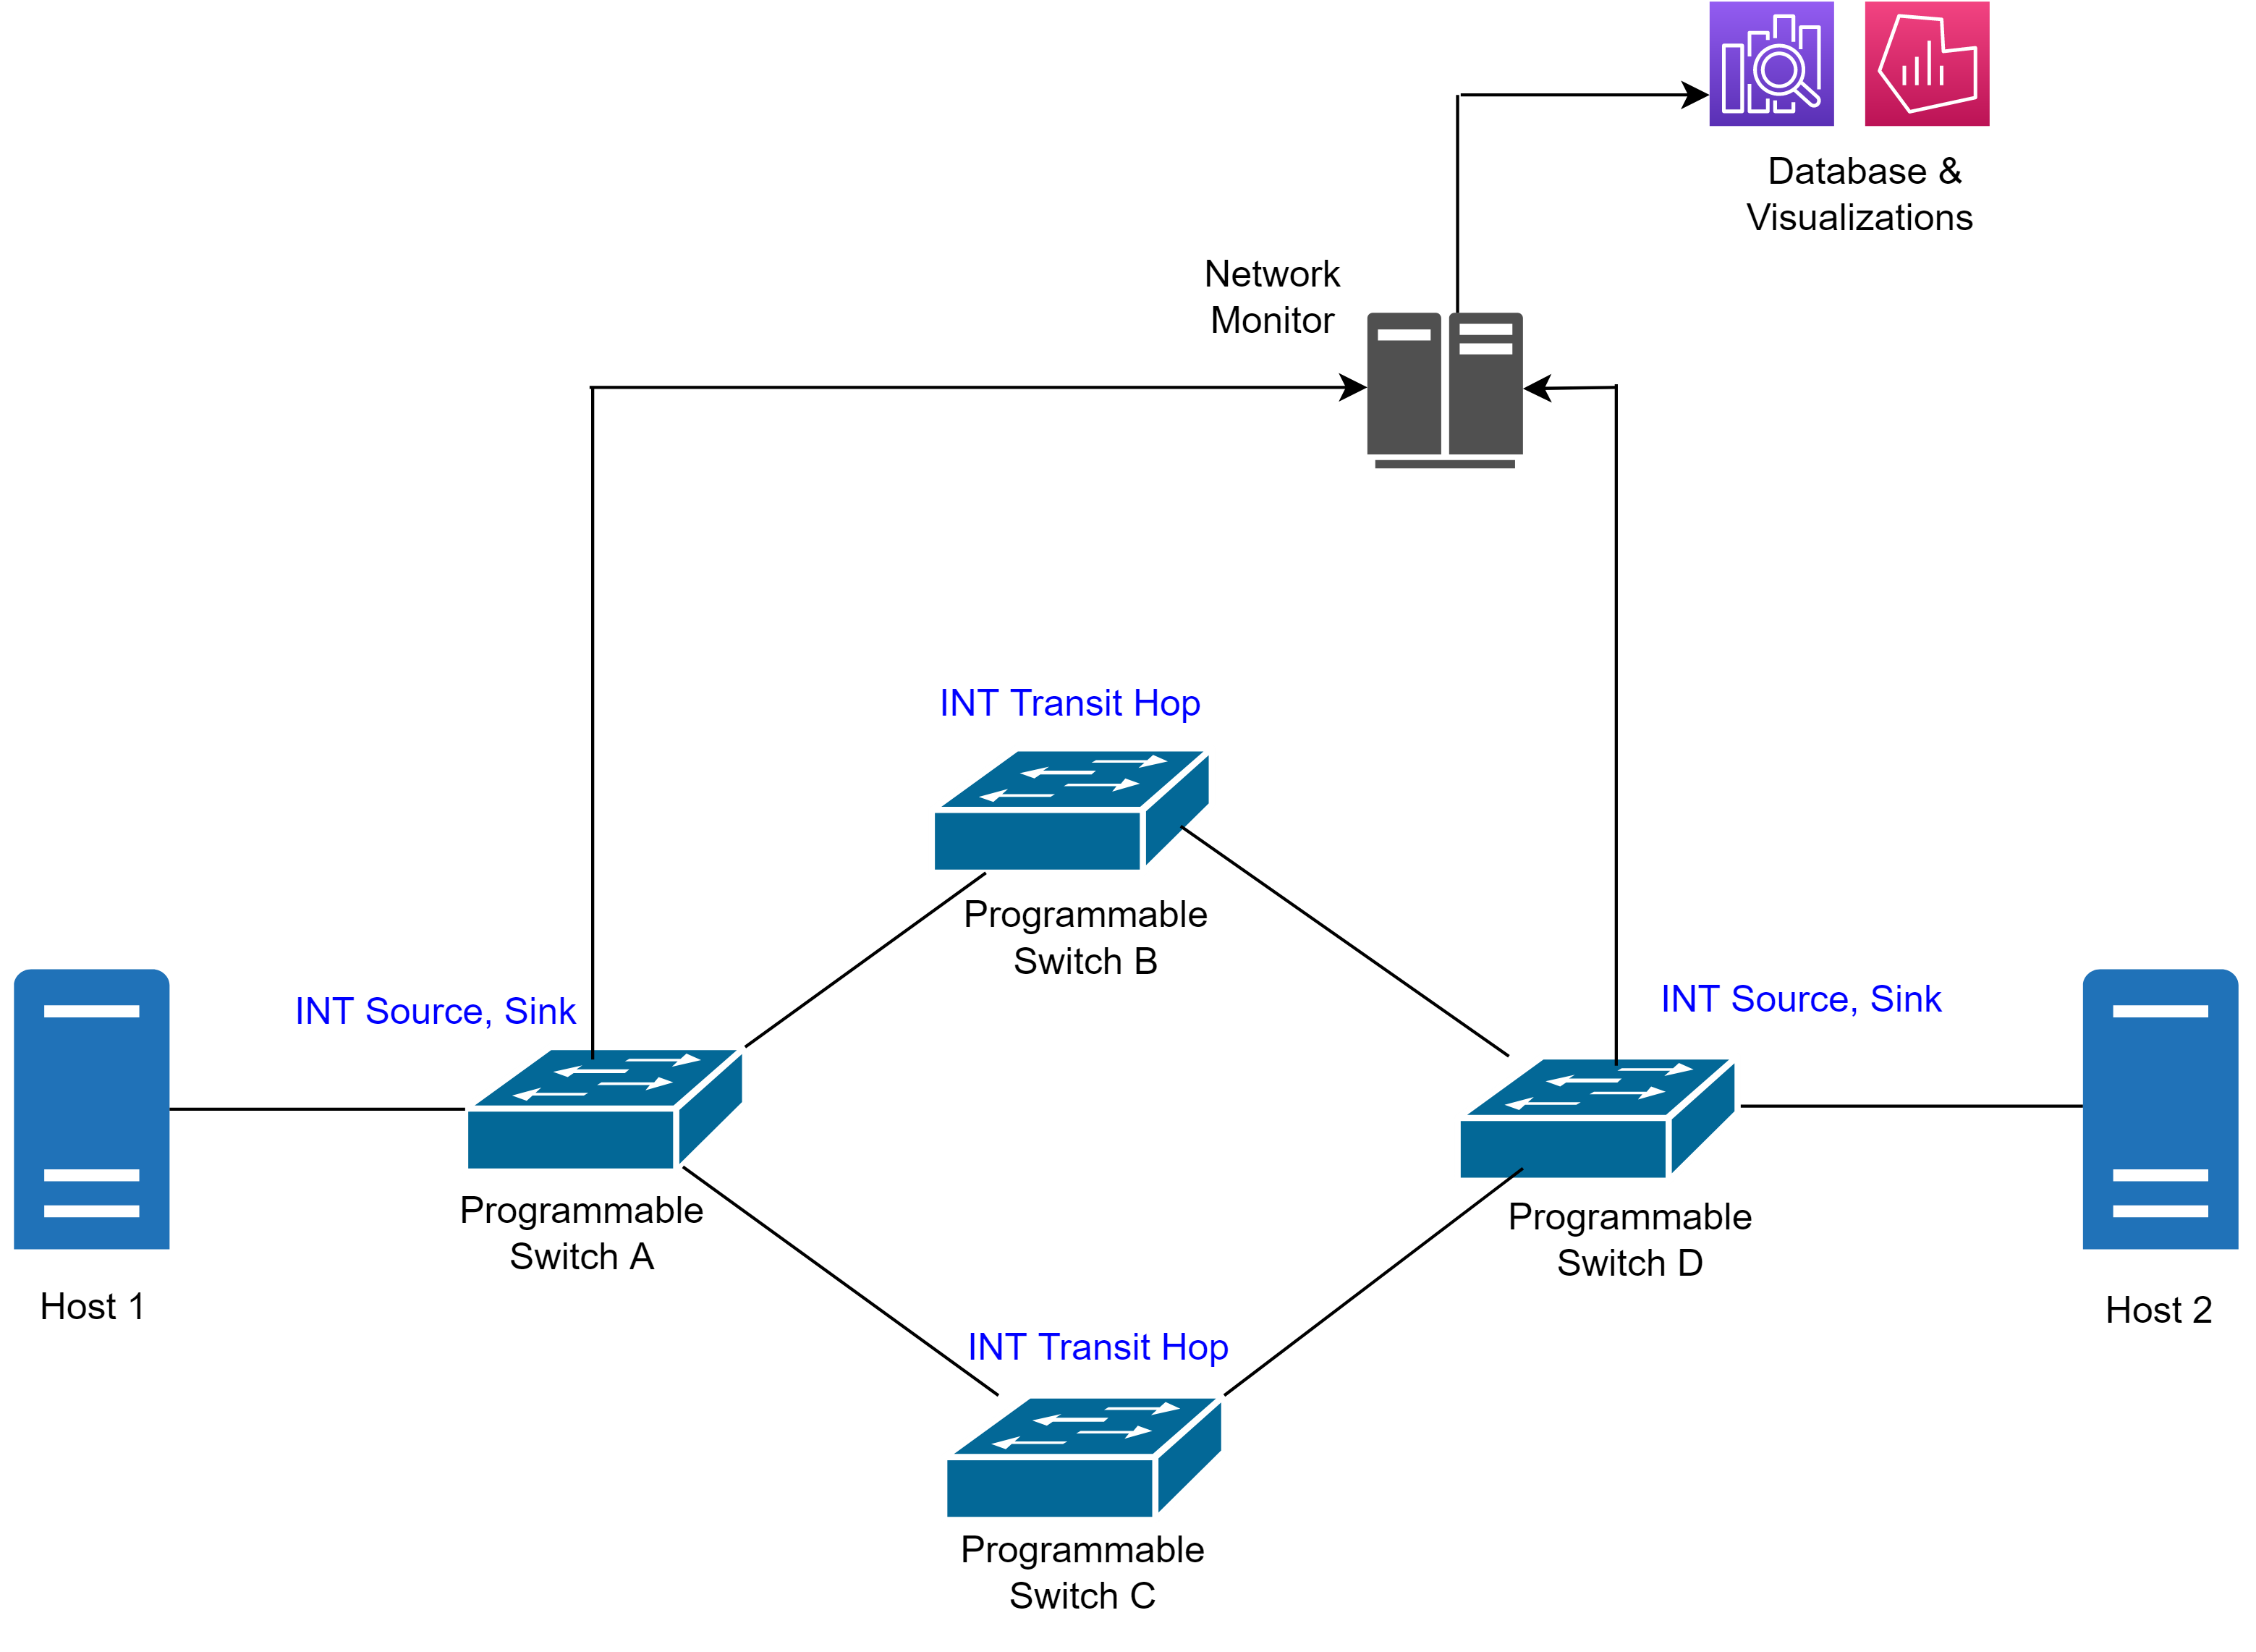
\includegraphics[scale=0.46]{Project_Proposal_Topology.png}}
	\caption{Experiment Slice Topology}
	\label{fig}
\end{figure*} 

\subsection{The INT Framework}
The final step is configuring the INT Framework to the entire slice topology mentioned. Each switch's roles are enhanced in this scenario to instantiate, forward, or collect INT Packets. Each INT Packet is configured to gather specified metadata of the data plane based on the INT instructions. The modified roles of the switches are illustrated in blue in Figure 1. Metrics such as hop latency and buffer queue time on the switch will be collected and sent to the Network Monitor for further processing and storage. \\
The primary challenge in setting up the INT-based Telemetry System is to minimize network \& processing overheads of the INT Packets while still collecting sufficient metrics to represent the flow state of the network accurately.

\section{Project Deliverables}
\subsection{Primary Objectives}
\begin{enumerate}
\item Walkthrough of P4 tutorials; implementing and deploying a basic P4 program on FABRIC.
\item Setting up the proposed topology on FABRIC. 
\item Implementing the entire telemetry system with minimal network and processing overheads and visualizing the telemetry gathered when the hosts communicate. This stage will also include writing a codebase using the MFLib API to continuously monitor and log slice information.
\item Deploy P4 Instructions to re-configure routing tables present in the switches in real-time.
\item Visualize the telemetry and slice information based on overall throughput and latency. We will also attempt to visualize a simulation showcasing the dynamic route-switching capability.
\end{enumerate}
\subsection{Stretch Objectives}
\begin{enumerate}
\item Implement the INT-based Telemetry System to monitor the entire slice topology.
\item Collect and visualize the metrics and logs gathered using the INT Packets, P4 Switches, and the Network Monitor.
\item Provide comparisons of the metrics gathered between the FABRIC Measurement Framework and the INT Framework. 
\end{enumerate}

\section{Learning Outcomes}
Our primary goal from this project is to gain a deep understanding of P4, its implementation details, and how to deploy P4 programs for data plane programmability. Our interest in P4 and the INT Framework stems from an appreciation for Dynamic Routing protocols and real-time Load Balancing systems. This project, if successful, could give us more insights into these core Networking topics.


\begin{thebibliography}{00}
\bibitem{b1} Pat Bosshart, Dan Daly, Glen Gibb, Martin Izzard, Nick McKeown, Jennifer Rexford, Cole Schlesinger, Dan Talayco, Amin Vahdat, George Varghese, and David Walker. 2014. “P4: programming protocol-independent packet processors”. SIGCOMM Comput. Commun. Rev. 44, 3 (July 2014), 87–95

\bibitem{b2} Weverton Luis da Costa Cordeiro, Jonatas Adilson Marques, Luciano Paschoal Gaspary, “Data Plane Programmability Beyond OpenFlow: Opportunities and Challenges for Network and Service Operations and Management.” Journal of Network and Systems Management (September 2017).

\bibitem{b3} Ilya Baldin, Anita Nikolich, Paul Ruth, Jim Griffioen, Kuang-Ching Wang, Inder Monga, and Tom Lehman, “FABRIC Measurement Framework Design,” v0.2

\bibitem{b4} The P4.org Applications Working Group. Contributions from Alibaba, Arista, CableLabs, Cisco Systems, Dell, Intel, Marvell, Netronome, VMware, “In-band Network Telemetry (INT) Dataplane Specification,” Version 2.1, 2020-11-11

\bibitem{b5} N. Van Tu, J. Hyun, and J. W.-K. Hong, "Towards ONOS-based SDN monitoring using in-band network telemetry," in Proc. 19th Asia–Pacific Netw. Oper. Manage. Symp. (APNOMS), Seoul, South Korea, Sep. 2017, pp. 76–81

\bibitem{b6} N. V. Tu, J. Hyun, G. Y. Kim, J. -H. Yoo and J. W. -K. Hong, "INTCollector: A High-performance Collector for In-band Network Telemetry," 2018 14th International Conference on Network and Service Management (CNSM), 2018, pp. 10-18.
\end{thebibliography}

\end{document}